\documentclass{article}
\usepackage[utf8]{inputenc}
\usepackage{graphicx}
\usepackage{listings}
\usepackage{amsmath}
\usepackage{color}
\usepackage{hyperref} 
\usepackage{mathtools}
\usepackage[final]{pdfpages}
\definecolor{backcolour}{rgb}{0.95,0.95,0.92}
\definecolor{codegreen}{rgb}{0,0.6,0}
\definecolor{codegray}{rgb}{0.5,0.5,0.5}
\definecolor{codepurple}{rgb}{0.58,0,0.82}

\graphicspath{ {./image/} }
 
\title{COT-5615\\ Math for Intelligent Systems\\Assignment 5}
\author{AKASH SHINGTE\\UFID: 4874-1966}
\date{19\textsuperscript{th} November 2018}
\lstdefinestyle{mystyle}{
    backgroundcolor=\color{backcolour},
    numbers=left,
    commentstyle=\color{codegreen},
    keywordstyle=\color{magenta},
    numberstyle=\tiny\color{codegray},
    stringstyle=\color{codepurple},
    basicstyle=\footnotesize,
    breakatwhitespace=false,         
    breaklines=true,                 
    captionpos=b,                    
    keepspaces=true,                 
    numbers=left,                    
    numbersep=5pt,                  
    showspaces=false,                
    showstringspaces=false,
    showtabs=false,                  
    tabsize=2
}
\lstset{style=mystyle}
\begin{document}

\maketitle

\section{Lagrange parameters and optimization}
\section{Convolution Neural Nets}

The assignment was to repeat the tutorial at
\href{http://adventuresinmachinelearning.com/keras-tutorial-cnn-11-lines/}{Adventures in Machine Learning} and conduct the following experiments by configuring the following parameters
\begin{enumerate}
    \item Convolution window of size 3x3 and 9x9
    \item Non-linearities
    \begin{itemize}
        \item RELU
        \item Tanh
        \item sigmoid
    \end{itemize}
    \item Optimizers
    \begin{itemize}
        \item Adam 
        \item Stochastic Gradient Descent
    \end{itemize}
\end{enumerate}
Taking a cross product of the parameter setting we get, 
\begin{eqnarray*}
CWS = \{'3x3', '9x9'\} \\
NL = \{'Relu', 'Tanh'\}\\
O = \{'Adam','SGD'\}\\
\\
Product = \mathbf{CWS} \bigtimes \mathbf{NL} \bigtimes \mathbf{O}
\end{eqnarray*}
8 possiblities
\begin{table}[h!]
\begin{tabular}{llll}
\textit{\textbf{Index}} & \textit{\textbf{Window}} & \textit{\textbf{Non linearity}} & \textit{\textbf{Optimizer}} \\
1                       & 3x3                      & RELU                            & SGD                         \\
2                       & 3x3                      & RELU                            & Adam                        \\
3                       & 3x3                      & Tanh                            & SGD                         \\
4                       & 3x3                      & Tanh                            & Adam                        \\
5                       & 9x9                      & RELU                            & SGD                         \\
6                       & 9x9                      & RELU                            & Adam                        \\
7                       & 9x9                      & Tanh                            & SGD                         \\
8                       & 9x9                      & Tanh                            & Adam                       
\end{tabular}
\end{table}
\subsection{Results for each setting}
\begin{enumerate}
    \item Window=3x3; Non Linearity=RELU; Optimizer=SGD
    \begin{itemize}
        \item Output indicating time for convergence of optimizer
            \begin{verbatim}
Epoch 1/10
 - 67s 1ms/step-loss:1.1512-acc: 0.7294-val_loss:0.3652-val_acc: 0.8891
Epoch 2/10
 - 64s 1ms/step-loss:0.2964-acc: 0.9109-val_loss:0.2355-val_acc: 0.9305
Epoch 3/10
 - 62s 1ms/step-loss:0.2108-acc: 0.9374-val_loss:0.1582-val_acc: 0.9549
Epoch 4/10
 - 59s 992us/step-loss:0.1644-acc: 0.9521-val_loss:0.1345-val_acc: 0.9588
Epoch 5/10
 - 61s 1ms/step-loss:0.1355-acc: 0.9606-val_loss:0.1141-val_acc: 0.9672
Epoch 6/10
 - 60s 1ms/step-loss:0.1175-acc: 0.9653-val_loss:0.1064-val_acc: 0.9642
Epoch 7/10
 - 62s 1ms/step-loss:0.1039-acc: 0.9689-val_loss:0.0936-val_acc: 0.9722
Epoch 8/10
 - 62s 1ms/step-loss:0.0930-acc: 0.9723-val_loss:0.0960-val_acc: 0.9690
Epoch 9/10
 - 63s 1ms/step-loss:0.0858-acc: 0.9742-val_loss:0.0790-val_acc: 0.9739
Epoch 10/10
 - 66s 1ms/step-loss:0.0795-acc: 0.9762-val_loss:0.0711-val_acc: 0.9769
Test loss: 0.07114460799451917
Test accuracy: 0.9769
\end{verbatim}
\item Epoch Vs Accuracy curve\newline         
\includegraphics[width=10cm]{1.png}
\end{itemize}
\item Window=3x3; Non Linearity=RELU, Optimizer=Adam
\begin{itemize}
    \item Output indicating time for convergence of optimizer\newline
    \begin{verbatim}
Epoch 1/10
 - 72s 1ms/step-loss:0.1540-acc: 0.9532-val_loss:0.0450-val_acc: 0.9854
Epoch 2/10
 - 70s 1ms/step-loss:0.0441-acc: 0.9862-val_loss:0.0396-val_acc: 0.9880
Epoch 3/10
 - 70s 1ms/step-loss:0.0301-acc: 0.9908-val_loss:0.0358-val_acc: 0.9887
Epoch 4/10
 - 70s 1ms/step-loss:0.0217-acc: 0.9929-val_loss:0.0324-val_acc: 0.9883
Epoch 5/10
 - 71s 1ms/step-loss:0.0156-acc: 0.9949-val_loss:0.0325-val_acc: 0.9896
Epoch 6/10
 - 74s 1ms/step-loss:0.0122-acc: 0.9962-val_loss:0.0324-val_acc: 0.9906
Epoch 7/10
 - 74s 1ms/step-loss:0.0101-acc: 0.9965-val_loss:0.0334-val_acc: 0.9905
Epoch 8/10
 - 76s 1ms/step-loss:0.0096-acc: 0.9968-val_loss:0.0283-val_acc: 0.9916
Epoch 9/10
 - 79s 1ms/step-loss:0.0060-acc: 0.9980-val_loss:0.0307-val_acc: 0.9914
Epoch 10/10
 - 80s 1ms/step-loss:0.0073-acc: 0.9977-val_loss:0.0268-val_acc: 0.9921
Test loss: 0.02683705496957409
Test accuracy: 0.9921
\end{verbatim}
    \item Epoch vs Accuracy Curve\newline
    \includegraphics[width=10cm]{2.png}
\end{itemize}

\item Window=3x3; NonLinearity=Tanh; Optimizer=SGD
\begin{itemize}
    \item Output indicating time for convergence of optimizer\newline
    \begin{verbatim}
Epoch 1/10
 - 71s 1ms/step-loss:0.9974-acc: 0.7680-val_loss:0.4065-val_acc: 0.8929
Epoch 2/10
 - 71s 1ms/step-loss:0.3530-acc: 0.9019-val_loss:0.2869-val_acc: 0.9200
Epoch 3/10
 - 71s 1ms/step-loss:0.2759-acc: 0.9206-val_loss:0.2352-val_acc: 0.9335
Epoch 4/10
 - 70s 1ms/step-loss:0.2322-acc: 0.9321-val_loss:0.2013-val_acc: 0.9420
Epoch 5/10
 - 71s 1ms/step-loss:0.2004-acc: 0.9419-val_loss:0.1735-val_acc: 0.9500
Epoch 6/10
 - 71s 1ms/step-loss:0.1762-acc: 0.9489-val_loss:0.1536-val_acc: 0.9559
Epoch 7/10
 - 71s 1ms/step-loss:0.1568-acc: 0.9553-val_loss:0.1370-val_acc: 0.9610
Epoch 8/10
 - 71s 1ms/step-loss:0.1410-acc: 0.9603-val_loss:0.1228-val_acc: 0.9645
Epoch 9/10
 - 70s 1ms/step-loss:0.1283-acc: 0.9641-val_loss:0.1124-val_acc: 0.9687
Epoch 10/10
 - 70s 1ms/step-loss:0.1177-acc: 0.9671-val_loss:0.1044-val_acc: 0.9705
Test loss: 0.10441762720644474
Test accuracy: 0.9705
\end{verbatim}
    \item Epoch vs Accuracy Curve\newline
    \includegraphics[width=10cm]{3.png}
\end{itemize}

\item Window=3x3, Non Linearity=Tanh, Optimizer=Adam
\begin{itemize}
    \item Output indicating time for convergence of optimizer\newline
    \begin{verbatim}
Epoch 1/10
 - 75s 1ms/step-loss:0.1617-acc: 0.9507-val_loss:0.0687-val_acc: 0.9789
Epoch 2/10
 - 74s 1ms/step-loss:0.0618-acc: 0.9812-val_loss:0.0512-val_acc: 0.9835
Epoch 3/10
 - 75s 1ms/step-loss:0.0467-acc: 0.9854-val_loss:0.0636-val_acc: 0.9811
Epoch 4/10
 - 74s 1ms/step-loss:0.0367-acc: 0.9885-val_loss:0.0506-val_acc: 0.9847
Epoch 5/10
 - 74s 1ms/step-loss:0.0288-acc: 0.9907-val_loss:0.0478-val_acc: 0.9859
Epoch 6/10
 - 74s 1ms/step-loss:0.0204-acc: 0.9935-val_loss:0.0535-val_acc: 0.9843
Epoch 7/10
 - 74s 1ms/step-loss:0.0153-acc: 0.9948-val_loss:0.0526-val_acc: 0.9849
Epoch 8/10
 - 74s 1ms/step-loss:0.0143-acc: 0.9957-val_loss:0.0495-val_acc: 0.9878
Epoch 9/10
 - 74s 1ms/step-loss:0.0091-acc: 0.9970-val_loss:0.0586-val_acc: 0.9871
Epoch 10/10
 - 78s 1ms/step-loss:0.0099-acc: 0.9965-val_loss:0.0511-val_acc: 0.9888
Test loss: 0.05111657968914785
Test accuracy: 0.9888
\end{verbatim}
    \item Epoch vs Accuracy Curve\newline
    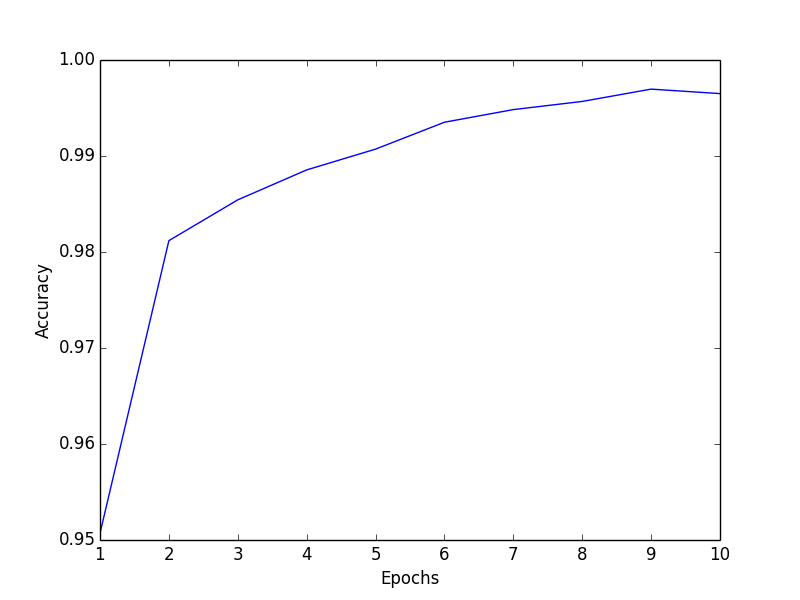
\includegraphics[width=10cm]{4.png}
\end{itemize}

\item Window=9x9; Non Linearity=RELU; Optimizer=SGD
\begin{itemize}
    \item Output indicating time for convergence of optimizer\newline
    \begin{verbatim}
Epoch 1/10
 - 61s 1ms/step-loss:1.7272-acc: 0.6022-val_loss:0.5929-val_acc: 0.8411
Epoch 2/10
 - 58s 963us/step-loss:0.4038-acc: 0.8865-val_loss:0.2862-val_acc: 0.9189
Epoch 3/10
 - 58s 965us/step-loss:0.2627-acc: 0.9230-val_loss:0.2172-val_acc: 0.9374
Epoch 4/10
 - 66s 1ms/step-loss:0.2133-acc: 0.9365-val_loss:0.1834-val_acc: 0.9453
Epoch 5/10
 - 58s 971us/step-loss:0.1831-acc: 0.9456-val_loss:0.1582-val_acc: 0.9540
Epoch 6/10
 - 59s 978us/step-loss:0.1625-acc: 0.9514-val_loss:0.1455-val_acc: 0.9579
Epoch 7/10
 - 59s 976us/step-loss:0.1448-acc: 0.9562-val_loss:0.1302-val_acc: 0.9616
Epoch 8/10
 - 63s 1ms/step-loss:0.1314-acc: 0.9606-val_loss:0.1204-val_acc: 0.9645
Epoch 9/10
 - 59s 981us/step-loss:0.1207-acc: 0.9635-val_loss:0.1062-val_acc: 0.9674
Epoch 10/10
 - 68s 1ms/step-loss:0.1112-acc: 0.9669-val_loss:0.1010-val_acc: 0.9707
Test loss: 0.10104400286264717
Test accuracy: 0.9707
\end{verbatim}
    \item Epoch vs Accuracy Curve\newline
    \includegraphics[width=10cm]{5.png}
\end{itemize}

\item Window=9x9; Non Linearity=RELU; Optimizer= Adam
\begin{itemize}
    \item Output indicating time for convergence of optimizer\newline
    \begin{verbatim}
Epoch 1/10
 - 70s 1ms/step-loss:0.2106-acc: 0.9370-val_loss:0.0636-val_acc: 0.9792
Epoch 2/10
 - 56s 938us/step-loss:0.0572-acc: 0.9824-val_loss:0.0487-val_acc: 0.9842
Epoch 3/10
 - 67s 1ms/step-loss:0.0383-acc: 0.9882-val_loss:0.0410-val_acc: 0.9869
Epoch 4/10
 - 58s 972us/step-loss:0.0281-acc: 0.9909-val_loss:0.0333-val_acc: 0.9903
Epoch 5/10
 - 59s 990us/step-loss:0.0231-acc: 0.9927-val_loss:0.0373-val_acc: 0.9881
Epoch 6/10
 - 54s 904us/step-loss:0.0190-acc: 0.9940-val_loss:0.0290-val_acc: 0.9903
Epoch 7/10
 - 48s 803us/step-loss:0.0162-acc: 0.9947-val_loss:0.0369-val_acc: 0.9896
Epoch 8/10
 - 57s 945us/step-loss:0.0125-acc: 0.9959-val_loss:0.0360-val_acc: 0.9904
Epoch 9/10
 - 47s 789us/step-loss:0.0120-acc: 0.9961-val_loss:0.0325-val_acc: 0.9900
Epoch 10/10
 - 45s 756us/step-loss:0.0105-acc: 0.9967-val_loss:0.0396-val_acc: 0.9902
Test loss: 0.03958743735278576
Test accuracy: 0.9902
\end{verbatim}
    \item Epoch vs Accuracy Curve\newline
    \includegraphics[width=10cm]{6.png}
\end{itemize}


\item Window=9x9; Non Linearity=Tanh; Optimizer=SGD
\begin{itemize}
    \item Output indicating time for convergence of optimizer\newline
    \begin{verbatim}
Epoch 1/10
 - 60s 1ms/step-loss:1.7258-acc: 0.5986-val_loss:0.7911-val_acc: 0.8397
Epoch 2/10
 - 57s 949us/step-loss:0.5162-acc: 0.8775-val_loss:0.3516-val_acc: 0.9104
Epoch 3/10
 - 56s 939us/step-loss:0.3118-acc: 0.9153-val_loss:0.2581-val_acc: 0.9280
Epoch 4/10
 - 56s 939us/step-loss:0.2456-acc: 0.9303-val_loss:0.2133-val_acc: 0.9384
Epoch 5/10
 - 57s 946us/step-loss:0.2085-acc: 0.9400-val_loss:0.1850-val_acc: 0.9467
Epoch 6/10
 - 57s 954us/step-loss:0.1828-acc: 0.9473-val_loss:0.1642-val_acc: 0.9525
Epoch 7/10
 - 57s 945us/step-loss:0.1634-acc: 0.9526-val_loss:0.1494-val_acc: 0.9561
Epoch 8/10
 - 58s 960us/step-loss:0.1481-acc: 0.9566-val_loss:0.1361-val_acc: 0.9598
Epoch 9/10
 - 49s 809us/step-loss:0.1352-acc: 0.9606-val_loss:0.1268-val_acc: 0.9621
Epoch 10/10
 - 52s 865us/step-loss:0.1244-acc: 0.9637-val_loss:0.1165-val_acc: 0.9658
Test loss: 0.11650260229483247
Test accuracy: 0.9658
\end{verbatim}
    \item Epoch vs Accuracy Curve\newline
    \includegraphics[width=10cm]{7.png}
\end{itemize}

\item Window=9x9; Non Linearity=Tanh; Optimizer=Adam
\begin{itemize}
    \item Output indicating time for convergence of optimizer\newline
\begin{verbatim}
Epoch 1/10
 - 60s 1ms/step-loss:0.2028-acc: 0.9395-val_loss:0.0889-val_acc: 0.9710
Epoch 2/10
 - 62s 1ms/step-loss:0.0664-acc: 0.9795-val_loss:0.0597-val_acc: 0.9801
Epoch 3/10
 - 62s 1ms/step-loss:0.0484-acc: 0.9850-val_loss:0.0430-val_acc: 0.9864
Epoch 4/10
 - 62s 1ms/step-loss:0.0350-acc: 0.9889-val_loss:0.0454-val_acc: 0.9861
Epoch 5/10
 - 63s 1ms/step-loss:0.0302-acc: 0.9901-val_loss:0.0440-val_acc: 0.9871
Epoch 6/10
 - 63s 1ms/step-loss:0.0246-acc: 0.9920-val_loss:0.0484-val_acc: 0.9854
Epoch 7/10
 - 61s 1ms/step-loss:0.0215-acc: 0.9926-val_loss:0.0528-val_acc: 0.9842
Epoch 8/10
 - 62s 1ms/step-loss:0.0188-acc: 0.9937-val_loss:0.0496-val_acc: 0.9853
Epoch 9/10
 - 61s 1ms/step-loss:0.0152-acc: 0.9949-val_loss:0.0475-val_acc: 0.9864
Epoch 10/10
 - 61s 1ms/step-loss:0.0169-acc: 0.9944-val_loss:0.0533-val_acc: 0.9866
Test loss: 0.053336763092613544
Test accuracy: 0.9866
\end{verbatim}
    \item Epoch vs Accuracy Curve\newline
    \includegraphics[width=10cm]{8.png}
\end{itemize}

\end{enumerate}
\end{document}
